\documentclass[conference]{IEEEtran}
\IEEEoverridecommandlockouts

\usepackage{cite}
\usepackage{amsmath,amssymb,amsfonts}
\usepackage{algorithmic}
\usepackage{graphicx}
\usepackage{textcomp}
\usepackage{xcolor}
\usepackage[T1]{fontenc}
\usepackage[utf8]{inputenc}
\usepackage[serbian]{babel}
\usepackage{dirtytalk}

\title{\textit{Brain computer interface},\\ mogućnosti primene (pregled)}

\author{\IEEEauthorblockN{Marija Gijić} \IEEEauthorblockA{{Fakultet tehničkih nauka}\\
{Univerzitet u Novom Sadu}\\
Novi Sad, Republika Srbija \\
marijagijic4@gmail.com} \\
\and
\IEEEauthorblockN{Sava Cvetković}
\IEEEauthorblockA{{Fakultet tehničkih nauka}\\
{Univerzitet u Novom Sadu}\\
Novi Sad, Republika Srbija \\
savacvetkovicking@gmail.com}\\
\and
\IEEEauthorblockN{Nemanja Manić}
\IEEEauthorblockA{{Fakultet tehničkih nauka}\\
{Univerzitet u Novom Sadu}\\
Novi Sad, Republika Srbija \\
nemanjamanic9@gmail.com}\\
\and
\IEEEauthorblockN{Marija Graovac}
\IEEEauthorblockA{{Fakultet tehničkih nauka}\\
{Univerzitet u Novom Sadu}\\
Novi Sad, Republika Srbija \\
graovacmarija2001@gmail.com}}

\begin{document}
\maketitle
\selectlanguage{serbian}
\begin{abstract}
U ovom radu opisani su osnovni pojmovi, principi rada \textit{Brain computer interface}-a i mogućnosti primene.
\end{abstract}
\textbf{\footnotesize\textit{Ključne reči}---BCI, akvizicija signala, primena, EEG, ECoG}

\section{Uvod}
\subsection{Definicija}
\textit{Brain computer interface} tehnologija (BCI) je moćan komunikacioni alat izme\dj u  korisnika i sistema. Predstavlja direktan komunikacioni put izme\dj u električne aktivnosti mozga i eksternog ure\dj aja, najčešće računara ili robotskog uda. Istraživačka zajednica je u početku razvijala BCI radi biomedicinskih primena što je rezultiralo stvaranju naprednijih medicinskih pomagala (ure\dj aja). Ovi ure\dj aji su olakšali svakodnevni život osobama koje imaju ograničeno kretanje i donekle zamenili izgubljene motoričke funkcionalnosti. Stručnija definicija bi bila: sistem koji uzima biosignal izmeren od osobe i predvi\dj a (u realnom vremenu) neki apstraktni aspekt neurološkog stanja osobe, kognitivno stanje, pažnju ili nameru. 
\begin{figure}[htp]
\centerline{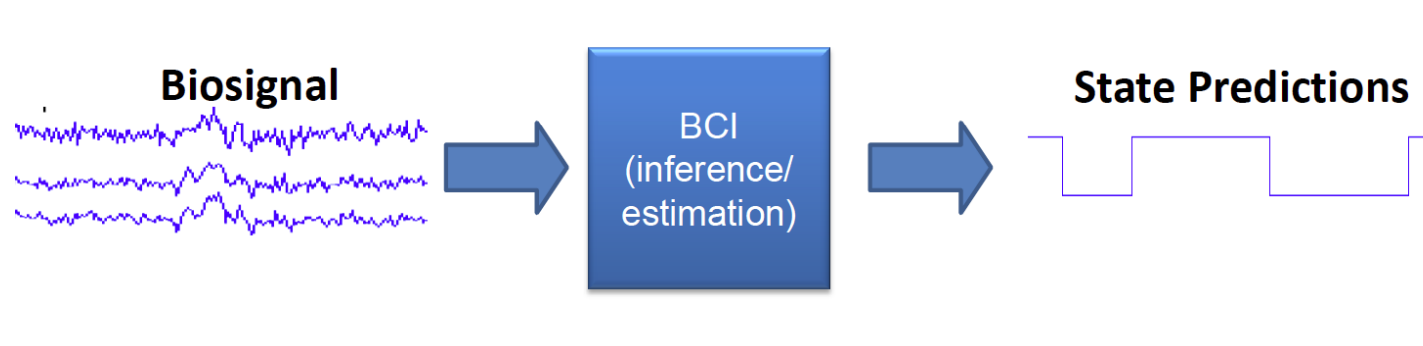
\includegraphics[width=8cm, height=2cm]{Biosignal.png}}
\caption{Predikcija biosignala}
\label{Slika}
\end{figure}
\subsection{Kriterijumi za BCI}
\begin{itemize}
\item Direktnost - sistem se mora oslanjati na direktne mere aktivnosti mozga
\item Realno vreme - realno vreme se odnosi na najviše jedan minut kašnjenja izme\dj u korisnikovog formiranja relevantne poruke ili komande i rezultujuće povratne informacije 
\item Povratna informacija - BCI mora da pruži u realnom vremenu povratnu infromaciju korisniku, odnosno, sistem mora da deluje prema nameri korisnika da bi korisnik mogao da zna da li je uspešno preneo željenu poruku ili komandu
\item Namera - korisnik mora da izvrši nešto dobrovoljno, namerno, da ciljano usmeri mentalnu aktivnost svaki put kada on/ona želi da prenese informaciju. 
\end{itemize}
\subsection{Vrste BCI-a}
\begin{itemize}
    \item Aktivni BCI (\textit{Brain-Machine Interface}) - BCI izvodi svoje izlaze na osnovu moždane aktivnosti kojom direktno i svesno kontroliše korisnik, nezavisno od spoljnih doga\dj aja
    \item Reaktivni BCI - BCI izvodi svoje izlaze na osnovu moždane aktivnosti koja nastaje kao reakcija na spoljašnju stimulaciju koja je indirektno modulisana od strane korisnika 
    \item Pasivni ili afektivni BCI - BCI izvodi svoje izlaze iz spontane moždane aktivnosti 
\end{itemize}
Podela BCI-a se može zasnivati na elektrodama koje se koriste za merenje moždane aktivnosti:
\begin{itemize}
    \item Neinvazivni BCI gde se elektrode postavljaju direktno na skalp (EEG, MEG, EOG, MRI)
    \item Invazivni BCI gde su elektrode direktno pričvršćene za mozak (ECoG (elektrokortikografija), iEEG (intrakranijalna elektroencefalografija))
\end{itemize}
\section{Princip rada BCI-a}
Svrha BCI-a je da otkrije i kvantifikuje karakteristike moždanih signala koji ukazuju na namere korisnika i da iste prevede u realnom vremenu u komande koje se zadaju ure\dj aju. Da bi se to postiglo, \textit{Brain computer interface} se sastoji od 4 sekvencijalne komponente:
\begin{itemize}
    \item akvizicija signala
    \item izdvajanje karakteristika moždanih signala
    \item prevo\dj enje
    \item izlaz ure\dj aja
\end{itemize}
Ove 4 komponente su kontrolisane operativnim protokolom koji definiše početak i tajming rada, detalje obrade signala, komande ure\dj aja, i nadozor performansa. Efikasni operativni protokol omogućava BCI sistemu fleksibilnosti odnosno da se prilago\dj ava specifičnim potrebama svakog korisnika.
\begin{figure}[htp]
\centerline{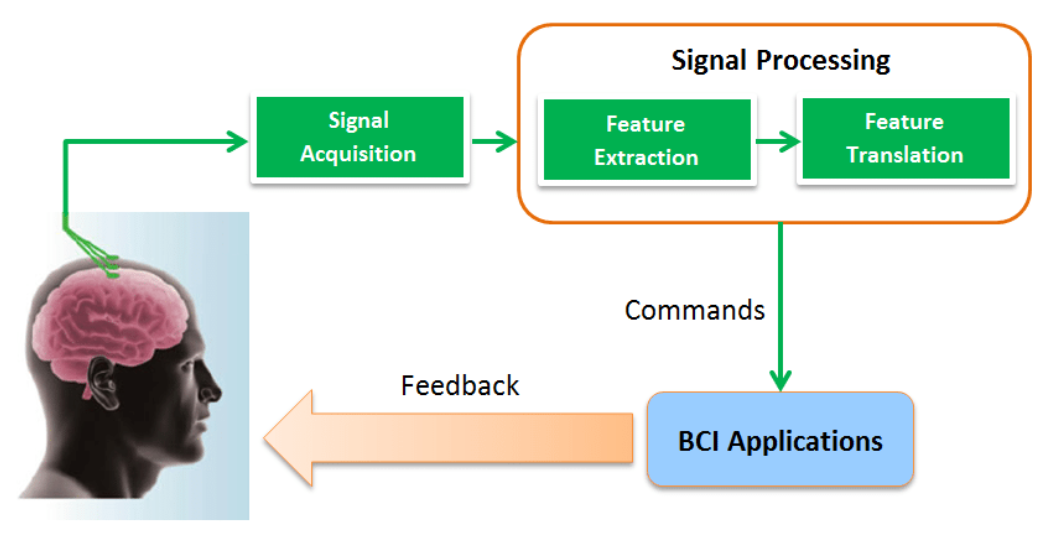
\includegraphics[width=8cm, height=4cm]{BCI-functions.png}}
\caption{Princip rada BCI-a}
\label{Slika}
\end{figure}
\subsection{Akvizicija signala}
Akvizicija signala je merenje moždanih signala korišćenjem odre\dj enog senzorskog mehanizma (npr. skalp ili intrakranijalne elektrode za elektrofiziološku aktivnost, fMRI (\textit{Functional magnetic resonance imaging}) za metaboličku aktivnost). Signali se pojačavaju do nivoa koji je pogodan za elektronsku obradu (i mogu tako\dj e biti podvrgnuti filtriranju da bi se uklonio električni šum ili druge nepoželjne karakteristike signala, kao npr. 60Hz smetnje u dalekovodu). Signali su tad digitalizovani i preneti na računar. 
\subsection{Izdvajanje karakteristika moždanih signala}
Izdvajanje karakteristika moždanih signala je proces analize digitalnih signala koji se sastoji od izdvajanja relevantne karakteristike signala (tj. karakteristike signala koje se odnose na nameru osobe) od stranog sadržaja i predstavljanja tih signala u pogodnom obliku za prevod u izlazne komande. Ove karakteristike treba da imaju jake korelacije sa namerom korisnika. Zbog velikog dela relevantne (tj. u najjačoj korelaciji) moždane aktivnosti koja je ili prolazna ili oscilatorna, najčešće ekstrahovane karakteristike signala u današnjim BCI sistemima su amplitude u vremenu i vremensko kašnjenje odziva EEG-a ili ECoG-a, snaga unutar specifičnih EEG ili ECoG frekvencijskih opsega, ili brzina pokretanje pojedinačnih kortikalnih neurona. Smetnje okoline ili fiziološke smetnje kao što su elektromiografski signali se izbegavaju ili uklanjaju da bi se obezbedila tačnost merenja moždanog signala.
\subsection{Prevo\dj enje}
Rezultujuće karakteristike signala se zatim prosle\dj uju na algoritam za prevo\dj enje funkcija, koji pretvara funkcije u odgovarajuće komande za izlazni ure\dj aj (tj. komande koje prate namere korisnika). Na primer, smanjenje snage u datom frekvencijskom opsegu bi se mogao prevesti u pomeranje naviše kursora računara. Algoritam prevo\dj enja treba da bude dinamičan da bi se prilagodio sponatnim ili naučenim promenama u karakteristikama signala i da bi se osiguralo da korisnikov mogući opseg vrednosti karakteristika pokriva ceo opseg kontrole ure\dj aja.
\subsection{Izlaz ure\dj aja}
Komande dobijene algoritmom za prevo\dj enje upravljaju eksternim ure\dj ajem pružajući funkcije kao što su izbor slova, kontrola kursora, rad robotske ruke i tako dalje. Rad ure\dj aja daje povratnu informaciju korisniku čime se zavtvara kontrolna petlja. 

\section{Tipovi BCI-a i njihove primene u medicini}
\subsection{BCI koji koriste EEG snimljen na skalpu}
Neinvazivni BCI zasnovani na EEG-u su najšire istraženog pristupa zbog minimalnog rizika i relativne pogodnosti sprovo\dj enja studija i regrutovanje ispitanika. Primene su do danas generalno ograničene na kontinuiranu kontrolu kretanja niskog stepena slobode i diskretnu selekciju. Senzomotorni ritmovi su korišćeni za kontrolu kursora u 1, 2 i 3 dimenzije, ure\dj aje za pravopis, konvencionalne pomoćne ure\dj aje, ortoze za ruke, funkcionalnu električnu stimulaciju (FES) ruke pacijenta, robotske i protetičke ure\dj aje i invalidska kolica.\\
\subsubsection{P300 mind-speller}
Zbog relativno jednostavne implementacije i performansa, jedna od najistraženijih BCI paradigmi je vizuelni P300 speler (\textit{Visual P300 mind-speller (VP3S)}) koji se uspešno pokazao i kod zdravih i kod osoba sa invaliditetom za kucanje, pretraživanje interneta, upravljanjem invalidskim kolicima po unapred odre\dj enim putanjama, i druge primene.\\
\\
\textit{P300 potencijal u vezi sa doga\dj ajem (P300 Event-Related Potential)}\\
\\
Me\dj u različitim EEG signalima, potencijali u vezi sa doga\dj ajima (ERPs) se odnose na skup moždanih signala koji se generišu u odgovor na neke spoljašnje stimuluse (vizuelne, slušne ili somatosenzorne). Na osnovu karakteristika signala ERP-ovi mogu biti kategorisani kao prolazni ili trajni. Prvi tip odgovara kratkotrajnim signalima koji se javljaju nakon odre\dj enog kašnjenja od početka događaja (P300), dok drugi tip obuhvata kontinuirane signale koji se generišu kao odgovor na neprekidni stimulus (vizuelno izazvan potencijal u stabilnom stanju). Zbog prirode ERP-ova (\textit{event-driven}), BCI zasnovani na njima spadaju u kategoriju reaktivnih sistema koji zahtevaju pažljivo osmišljavanje stimulusa.\\
P300 je istaknuta prolazna ERP komponenta koju karakteriše endogena pozitivna defleksija u EEG-u koja se javlja oko 300 ms nakon specifičnog stimulusa (vizualnog, slušnog ili somatosenzornog). To može da izazove \say{oddball} paradigmu u kojoj je subjekt izložen dvema vrstama ponovljenih stimulusa: jedan se javlja retko ili neučestano (poznat kao ciljni stimulus), a drugi često ili učestano (poznat kao neciljani stimulus). Slika 3 predstavlja grafik P300 talasa (označen u pravougaoniku), izazvan neučestanim vizuelnim stimulusom. Kao što se vidi na slici, amplituda talasa P300 je mnogo veća u pore\dj enju sa EEG odgovorima na učestane stimuluse. Amplituda i latencija P300 talasa zavise od subjekta. Preciznije, amplituda talasa ima pozitivnu vezu sa neizvesnošću pojava ciljanih stimulusa dok latencija zavisi od vremena koje je potrebno subjektu da kognitivno proceni ciljani stimulus. Me\dj u BCI baziranim na prolaznim ERP-ovima, P300 sistemi su privukli veću pažnju istživačima zbog njihove srazmerno bolje tačnosti i pouzdanosti.\\
\begin{figure}[htp]
\centerline{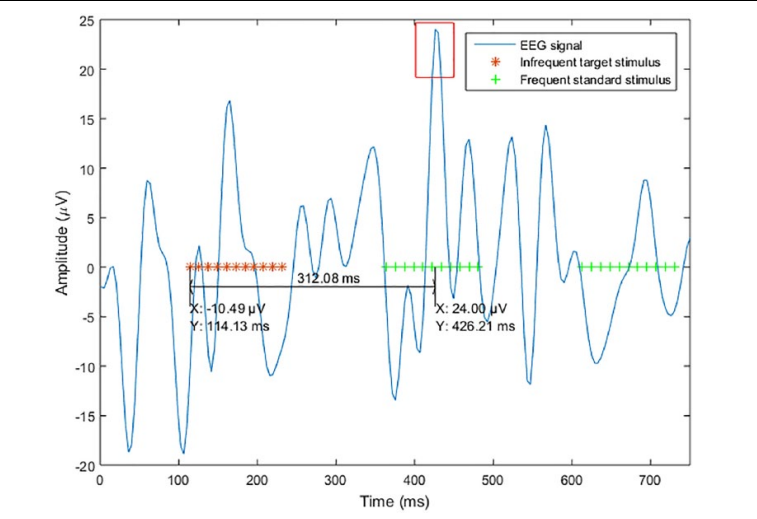
\includegraphics[width=9cm, height=5cm]{P300 signal.png}}
\caption{Vizuelna P300 komponenta (u pravougaoniku)}
\label{Slika}
\end{figure}
\\
\\
\textit{Akvizicija P300}\\
\\
EEG signali sa skalp elektroda oko centralnih i parientalnih regija mozga imaju najjaču i pouzdanu ERP distribuciju i stoga se obično koriste za datekciju P300 komponente. Većina konvencionalnih sistema zasnovanih na P300 koriste najmanje 3 skalp elektrode koje se nalaze na Fz, Cz  i Pz lokacijama 10-20 internacionalnog pozicionog sistema elektroda. Indetifikovano je da su elektrode na pozicijama Cz, Pz, Oz, PO7 i PO8 koje odgovaraju parijentalnoj i okcipitalnoj regiji mozga relevantne za detekciju P300 komponente kod normalnih subjekta. Kasnije je otkriveno da su elektrone na Cz i CP4 pozicijama relevantne u VP3S za pacijente sa amiotrofičnom lateralnom sklerozom (ALS).
\begin{figure}[htp]
\centerline{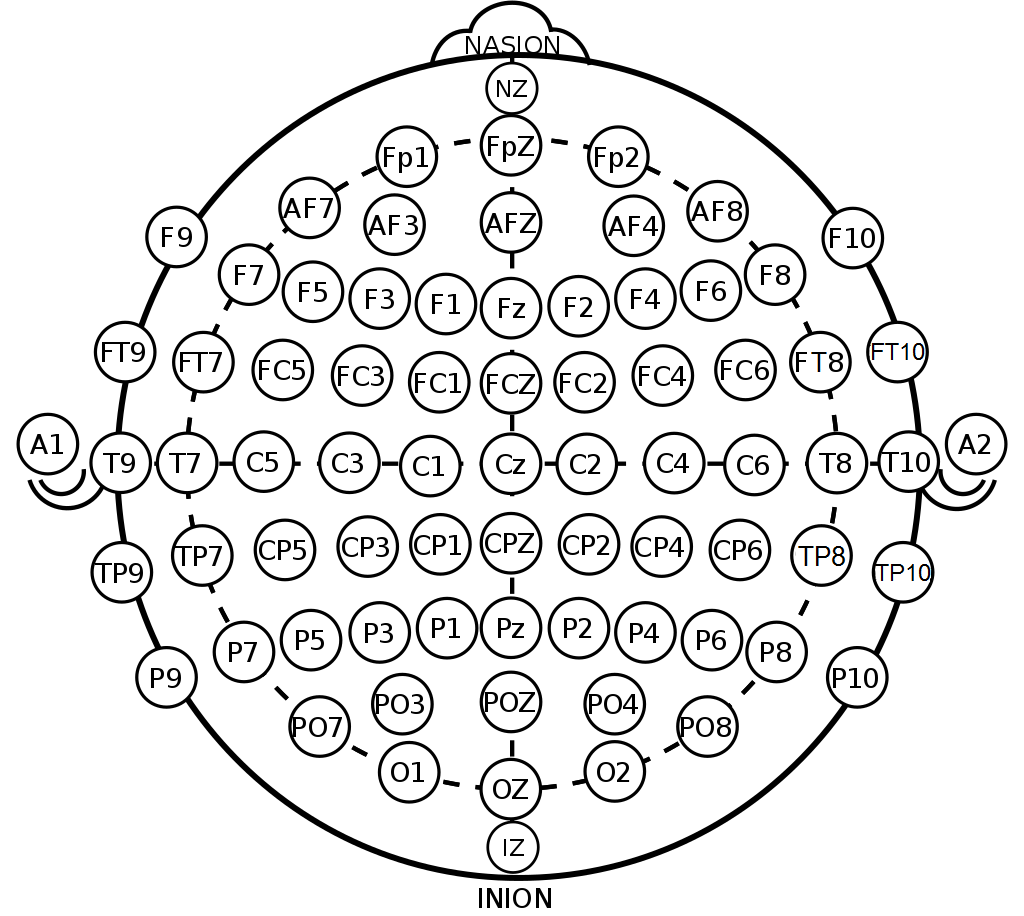
\includegraphics[width=6cm, height=5cm]{International_10-20_system_for_EEG-MCN.png}}
\caption{10-20 sistem}
\label{Slika}
\end{figure}
\\
\textit{Primena}
\\\\
\textit{Mind-speller} je široko istažena tema i opisana u literaturi o BCI baziranom na P300. Njegovoj popularnosti doprinose ogromne mogućnosti primene u kretanju i pomoći u komunikaciji, posebno za rehabilitaciju invalida. U zdravstvenom sektoru može pomoći delimično paralizovanim pacijentima kao što su ljudi koji boluju od ALS-a a i moždanog udara.
\\
Vizuelni P300 speler (VP3S) je BCI sistem koji olakšava indetifikaciju specifičnog izbora u umu subjekta iz skupa prikazanih elemenata (slova/simboli/slike). Sistem to postiže zadavanjem grupe vizuelno stimulusnih testova koji izazivaju signal P300 samo za elemente koje subjekt posmatra (tj. ciljni element). Tokom eksperimenta prikuplja EEG signal pomoću skalp elektroda i analizira ga. Otkrivanjem i lociranjem P300 komponente u EEG-u sistem može prepoznati element koji subjekt posmatra. VP3S se može rasporediti koristeći jednostavni matrični prikaz u složenim okruženjima virtuelne realnosti, čime se nudi prostor za širok spektar primena, posebno u medicinskim industrijama pa čak i u gejming industrijama.
\begin{figure}[htp]
\centerline{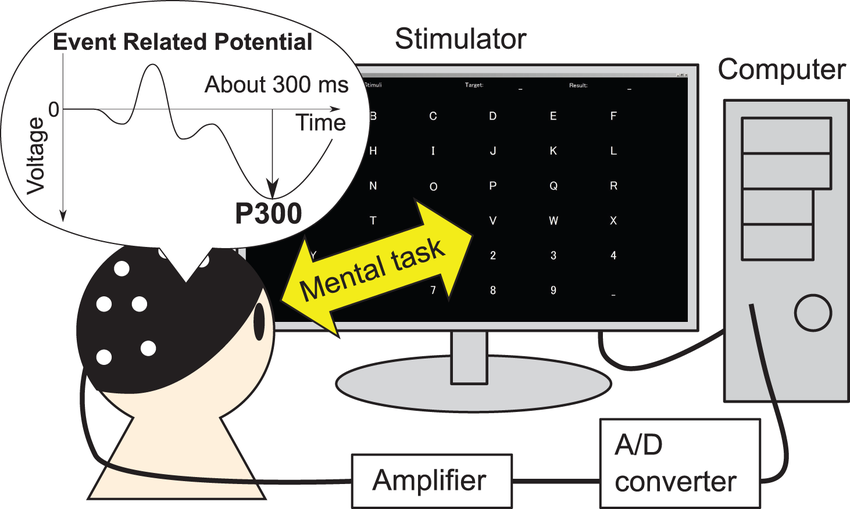
\includegraphics[width=9cm, height=5cm]{Structure-of-the-P300-based-BCI-system-A-target-letter-is-presented-to-a-participant.png}}
\caption{Struktura BCI sistema baziranog na P300}
\label{Slika}
\end{figure}
\subsubsection{Upotreba BCI u neurorehabilitaciji}
Upotreba BCI u neurorehabilitaciji je još uvek u procesu istraživanja. Hipoteza je da BCI mogu poboljšati trenutne rehabilitacione terapije tako što će ojačati oštećena područja mozga i veza i time povećati efikasnost njihove upotrebe. Studije kod pacijenata sa moždanim udarom su pokazale da se uz intervenciju ponovnog učenja motornih aktivnosti EEG karakteristike menjaju paralelno sa poboljšanjem motorike funkcija i da se senzomotornom rehabilitacijom korišćenjem BCI treninga i motoričkih slika može poboljšati motorička funkcija nakon povrede centralnog nervnog sistema. Kombinovanjem BCI-a sa FES-om (\textit{Functional Electrical Stimulation}) ili pomoćnim robotskim ure\dj ajima pomaže u obnavljanju motorike kod pacijenata sa moždanim udarom. Terapija zasnovana na BCI-u mogla bi pružiti korisni doprinos standardnim metodama neurorehabilitacije i može smanjiti potrebu za konstantnim nadozorom neurorehabilitacionog terapeuta.
\begin{figure}[htp]
\centerline{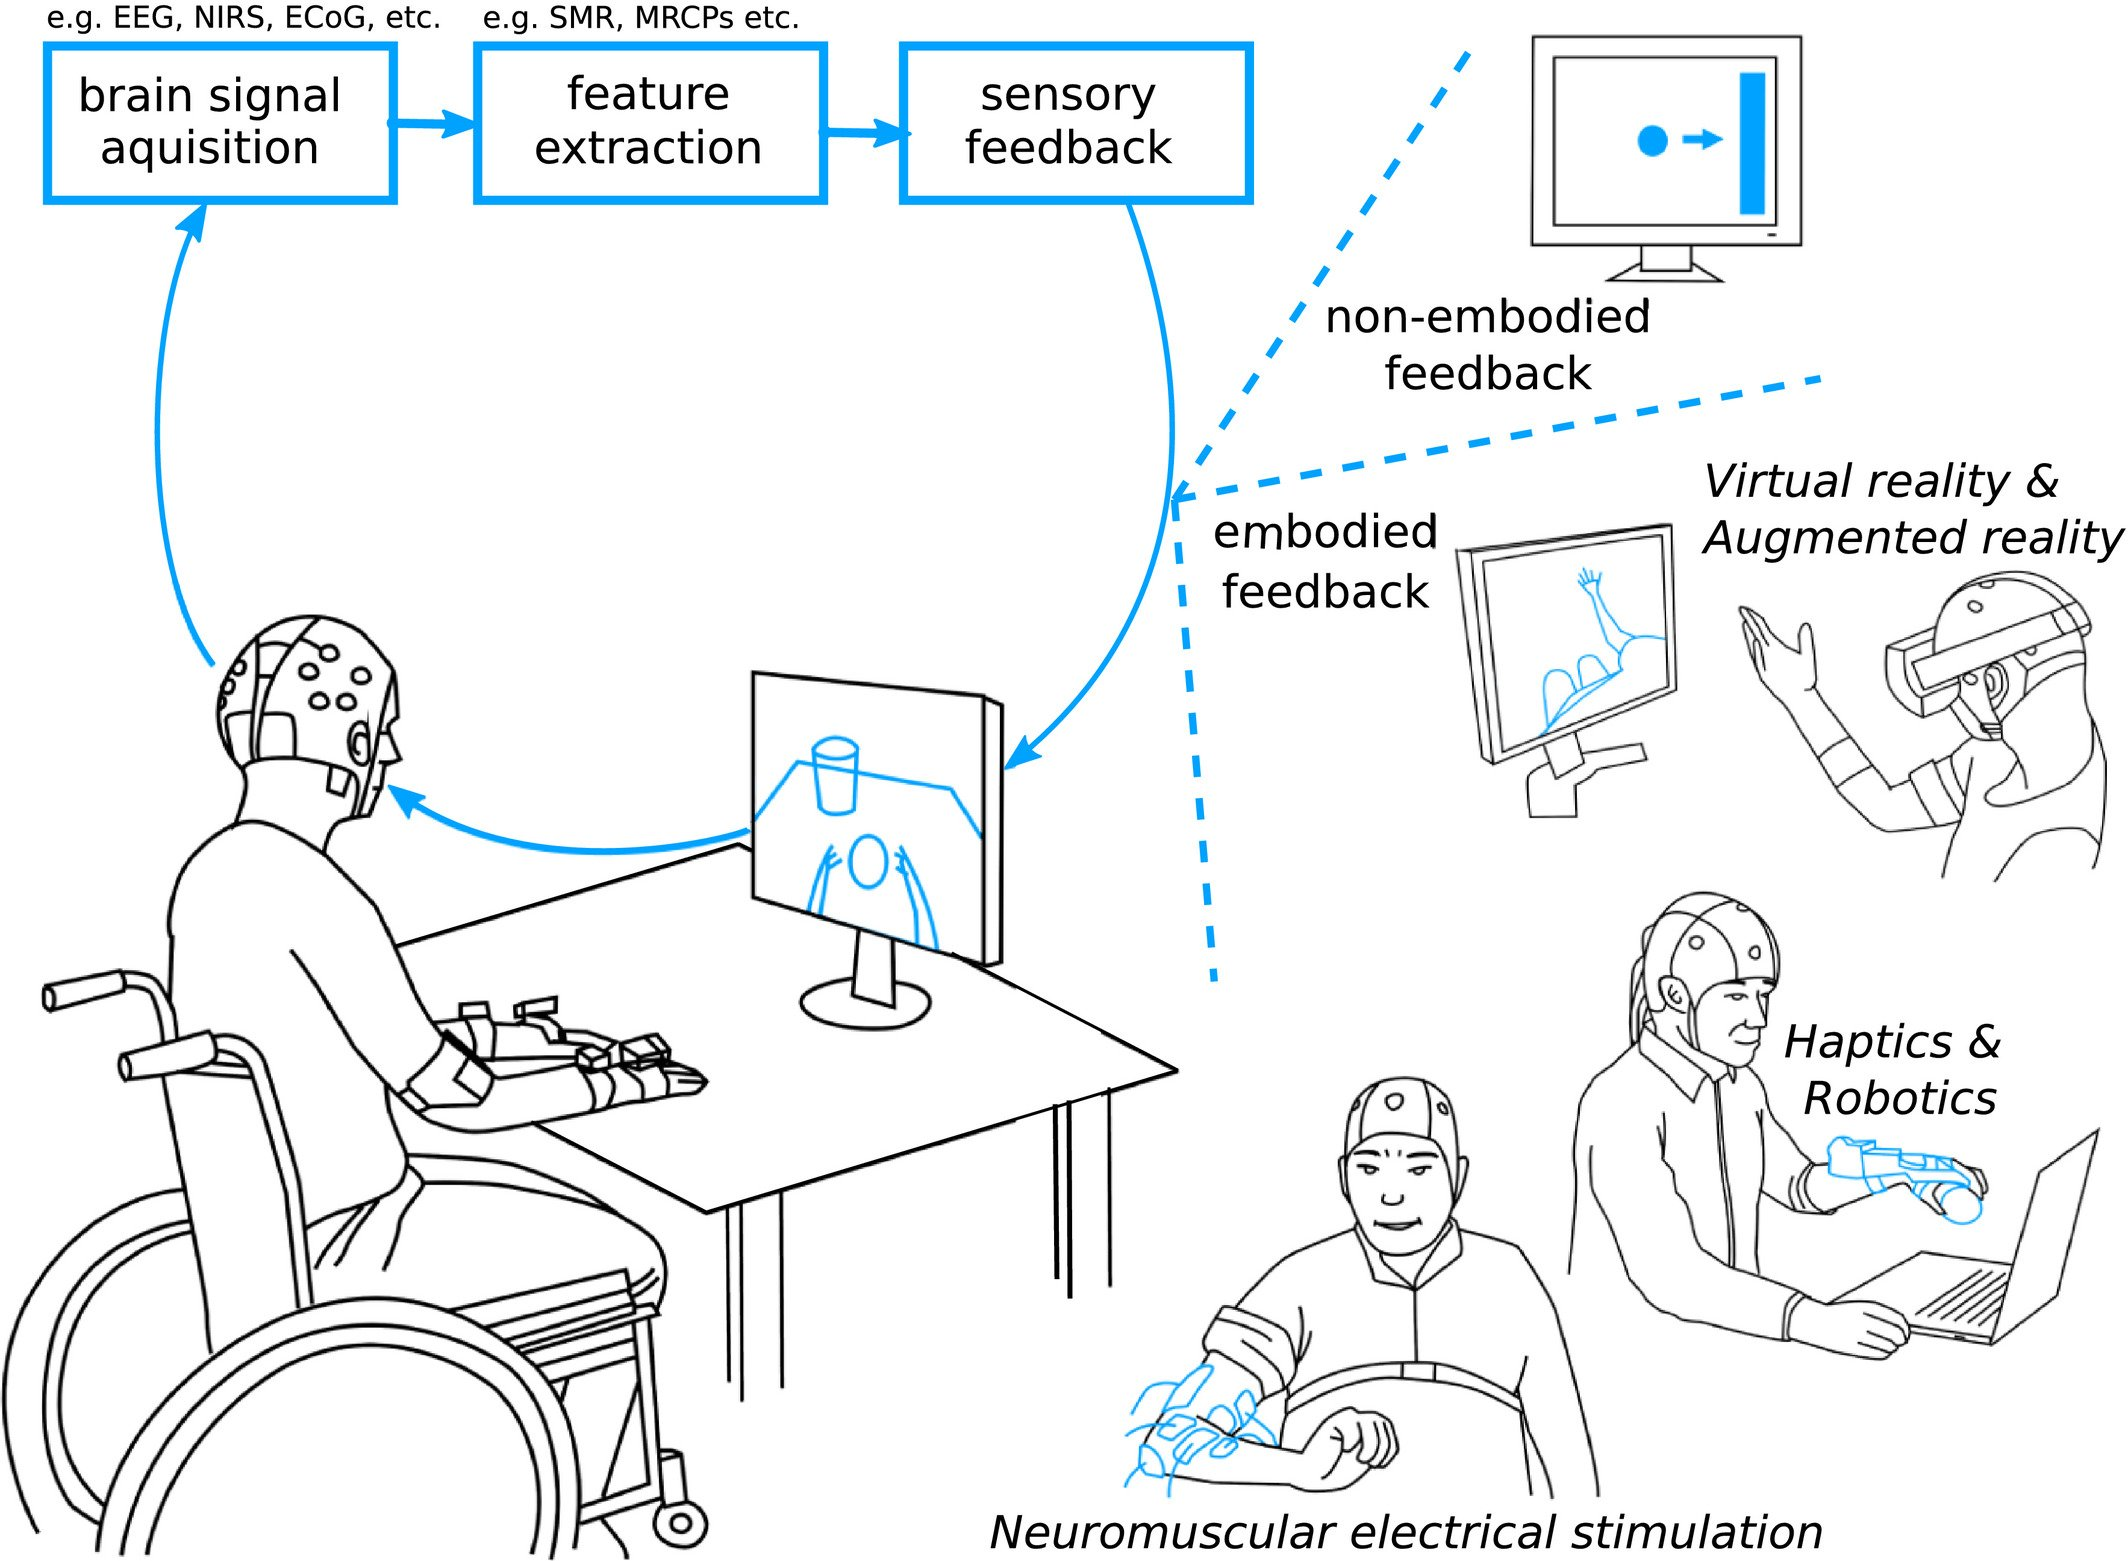
\includegraphics[width=6cm, height=4cm]{DZMaDzTWkAAdKzh.jpg}}
\caption{BCI u neurorehabilitaciji}
\label{Slika}
\end{figure}
\subsection{BCI koji koriste ECoG aktivnost}
Elektrokortikografija (ECoG), koja se tako\dj e ponekad naziva intrakranijalni EEG ili iEEG, je tehnika snimanja električnih signala sa lokacija ispod lobanje ali ne i unutar samog mozga. \\
\\
\textit{Akvizicija ECoG-a}\\
\\
ECoG aktivnost se može snimati sa površine dura mater (epiduralno) pomoću elektroda postavljenim na duru ili pomoću šrafova koji prodiru u lobanju i služe kao elektrode. Alternativno, ECoG se može snimiti i ispod dure (subduralno) pomoću postavljenih elektroda direktno na površini mozga. Elektrode se postavljaju tako da budu što bliže izvoru signala. \\
\begin{figure}[htp]
\centerline{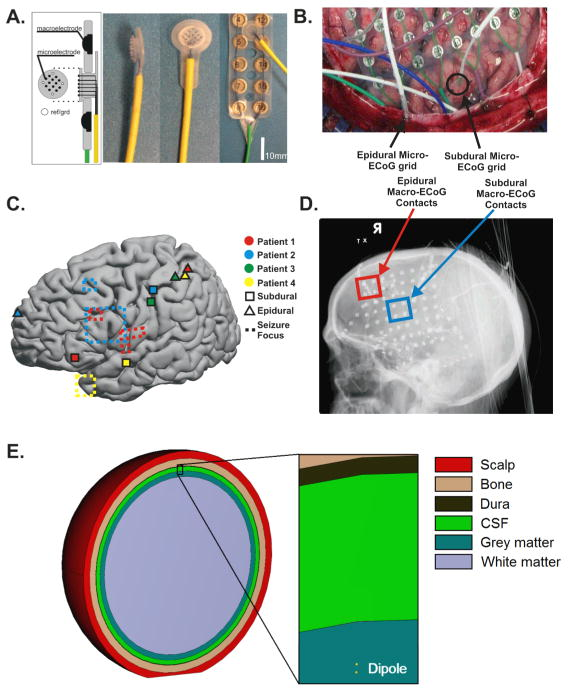
\includegraphics[width=7cm, height=6cm]{epi sub dural.jpg}}
\caption{Epiduralno (crveni kvadrat) i subduralno (plavi kvadrat) postavljanje elektroda}
\label{Slika}
\end{figure}\\
ECoG beleži signale većih amplituda i nudi superiorniju prostornu rezoluciju i sprektralni propusni opseg. Signal sa većom aplitudom znači da će manje biti pogođen šumom i artefaktima koji nastaju usled rada mišića.
\begin{figure}[htp]
\centerline{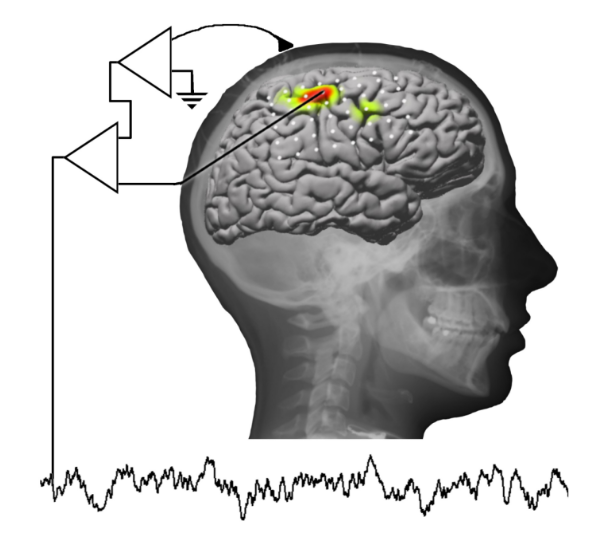
\includegraphics[width=5cm, height=5cm]{ECOG akv.png}}
\caption{Akvizicija ECoG-a}
\label{Slika}
\end{figure} 
U pore\dj enju sa aktivnostima nižih frekvencija (<40 Hz) koje su dominantne u EEG-u ECoG uključuje aktivnosti više frekvencije (>40 Hz gama opsega) do 200 Hz a moguće je i više od toga. Gama aktivnost je važna jer pokazuje veoma preciznu funkcionalnu lokalizaciju; u velikoj je korelaciji sa specifičnim aspektima motoričke, jezičke i kognitivne funkcije; i povezana je sa brzinom pojedinačnih neurona i signalima koji zavise od nivoa kiseonika u krvi koji detektuje fMRI (\textit{functional Magnetic Resonance Imaging}).\\
Istraživači su iskoristili ovo snimanje preko korteksa u više studija koje su se bavile motoričkim zadacima i klasifikacijom govornog procesa. Jedan od njih je koristio ECoG signale za predikciju kinematičkih parametara za petoklasnu fleksiju prstiju, dok je drugi odlikovao više parova motoričkih slika, kao što su pokreti leve naspram desne ruke, uz pomoć ECoG signala mozga i za paralizovane i pokretne epileptične pacijente. Tako\dj e je otkriveno da aktivnost pokretnih pacijenata može biti kategorizovana i shvaćena od strane sistema. 
\begin{figure}[htp]
\centerline{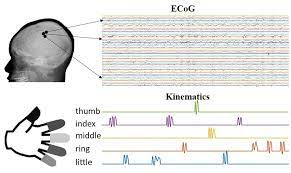
\includegraphics[width=7cm, height=4cm]{kontrola prst.jpg}}
\caption{Primer ECoG signala i ispitivanja kinematičkih parametara za petoklasnu fleksiju prstiju}
\label{Slika}
\end{figure}
\\
\textit{Elektrofiziološke karakteristike detektovane pomoću ECoG-a} \\
\\
Svojom detekcijom električne aktivnosti mozga u širokom frekvencijskom opsegu, ECoG detektuje nekoliko elektrofizioloških karakteristika koje BCI potencijalno može koristiti. To uključuje senzomotorne mu i beta ritmove. Senzomotorni mu ritmovi (ili mu talasi) su sihronizovani obrasci električne aktivnosti koji uključuje veliki broj neurona u delu mozga koji kontroliše voljno kretanje. Ovi obrasci se ponavljaju sa frekvencijom od 7.5-12.5 (i prvenstveno 9-11) Hz i najizraženiji su kada telo fizički miruje. Beta ritmovi (ili beta talasi) su neuronske oscilacije (moždani talasi) u mozgu sa frekvencijskim opsegom izme\dj u 12.5 i 30 Hz (12.5 do 30 ciklusa u sekundi). Beta stanja su povezana sa normalnom budnom svešću. \\
Promene u amplitudi mu ili  beta talasa obično se javljaju sa stvarnim ili zamišljenim pokretima (slika 10.), i relativno su spektralno fokusirani ali relativno prostorno rasprostranjeni (slika 11.). Amplituda mu ili beta talasa daje informaciju o opštim aspektima pokreta (na primer da li se ruka pomera ili ne) ali se smatra da sadrži vrlo skromne informacije o detaljima kretanja (npr. kinetički parametri pokreta ruku).\\
\\
\begin{figure}[htp]
\centerline{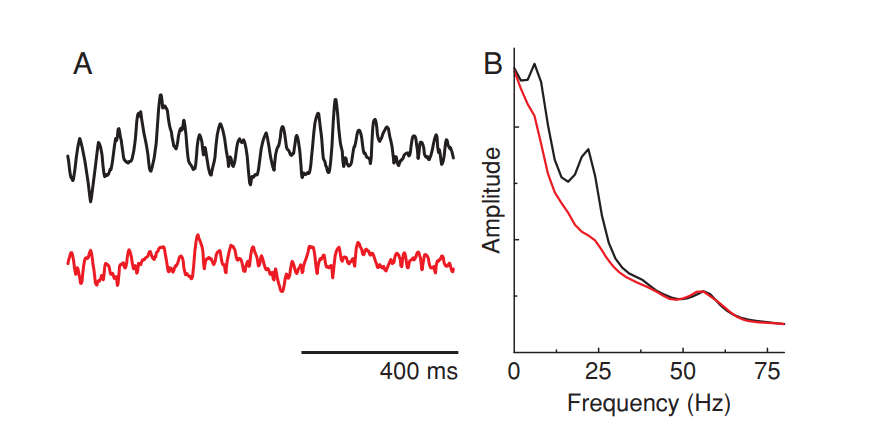
\includegraphics[width=7cm, height=4cm]{mu beta.png}}
\caption{Primer ECoG signala tokom zadatka i odmora. (A) Dobijen ECoG signal subjekta tokom odmora (crni signal) i dok zamišlja da izgovara reč „pomeriti” (crveni signal). (B) frekvencijski spektri povezani sa odgovarajućim uslovima. Slike su povezane sa smanjivanjem u mu i beta frekvcencijskim opsezima.}
\label{Slika}
\end{figure} \\
\begin{figure}[htp]
\centerline{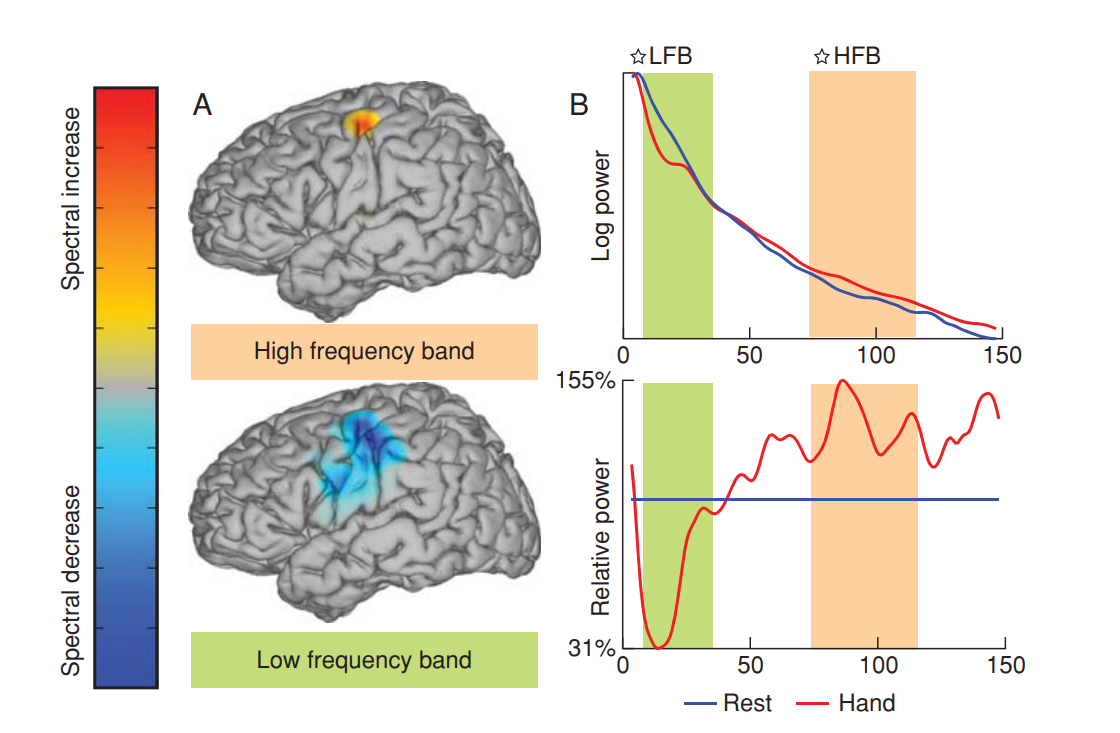
\includegraphics[width=8cm, height=4cm]{frekv ecog.png}}
\caption{Primer ECoG signala tokom zadatka ponavljanja otvaranja i zatvaranja šake i tokom odmora. (A) Signali u mu/beta opsegu (5-30 Hz) se smanjuju sa zadatkom i prostorno su manje specifični (tj. široko su topografski raspore\dj eni), dok signali u gama opsegu (tj. 70-116 Hz kako je izmereno ovde) se povećavaju sa zadatkom i prostorno su specifičniji (oštro su topografski fokusirani). (B) Spektar snage u logaritamskoj skali za elektrodu koja je označena zvezdicom na topografijama ilustruje smanjenje u mu/beta opsegu (zelena „traka”) i povećanje u gama opsegu (narandžasta „traka”)}

\label{Slika}
\end{figure}
\\
\\
\textit{Primena} \\
\\
\begin{figure}[htp]
\centerline{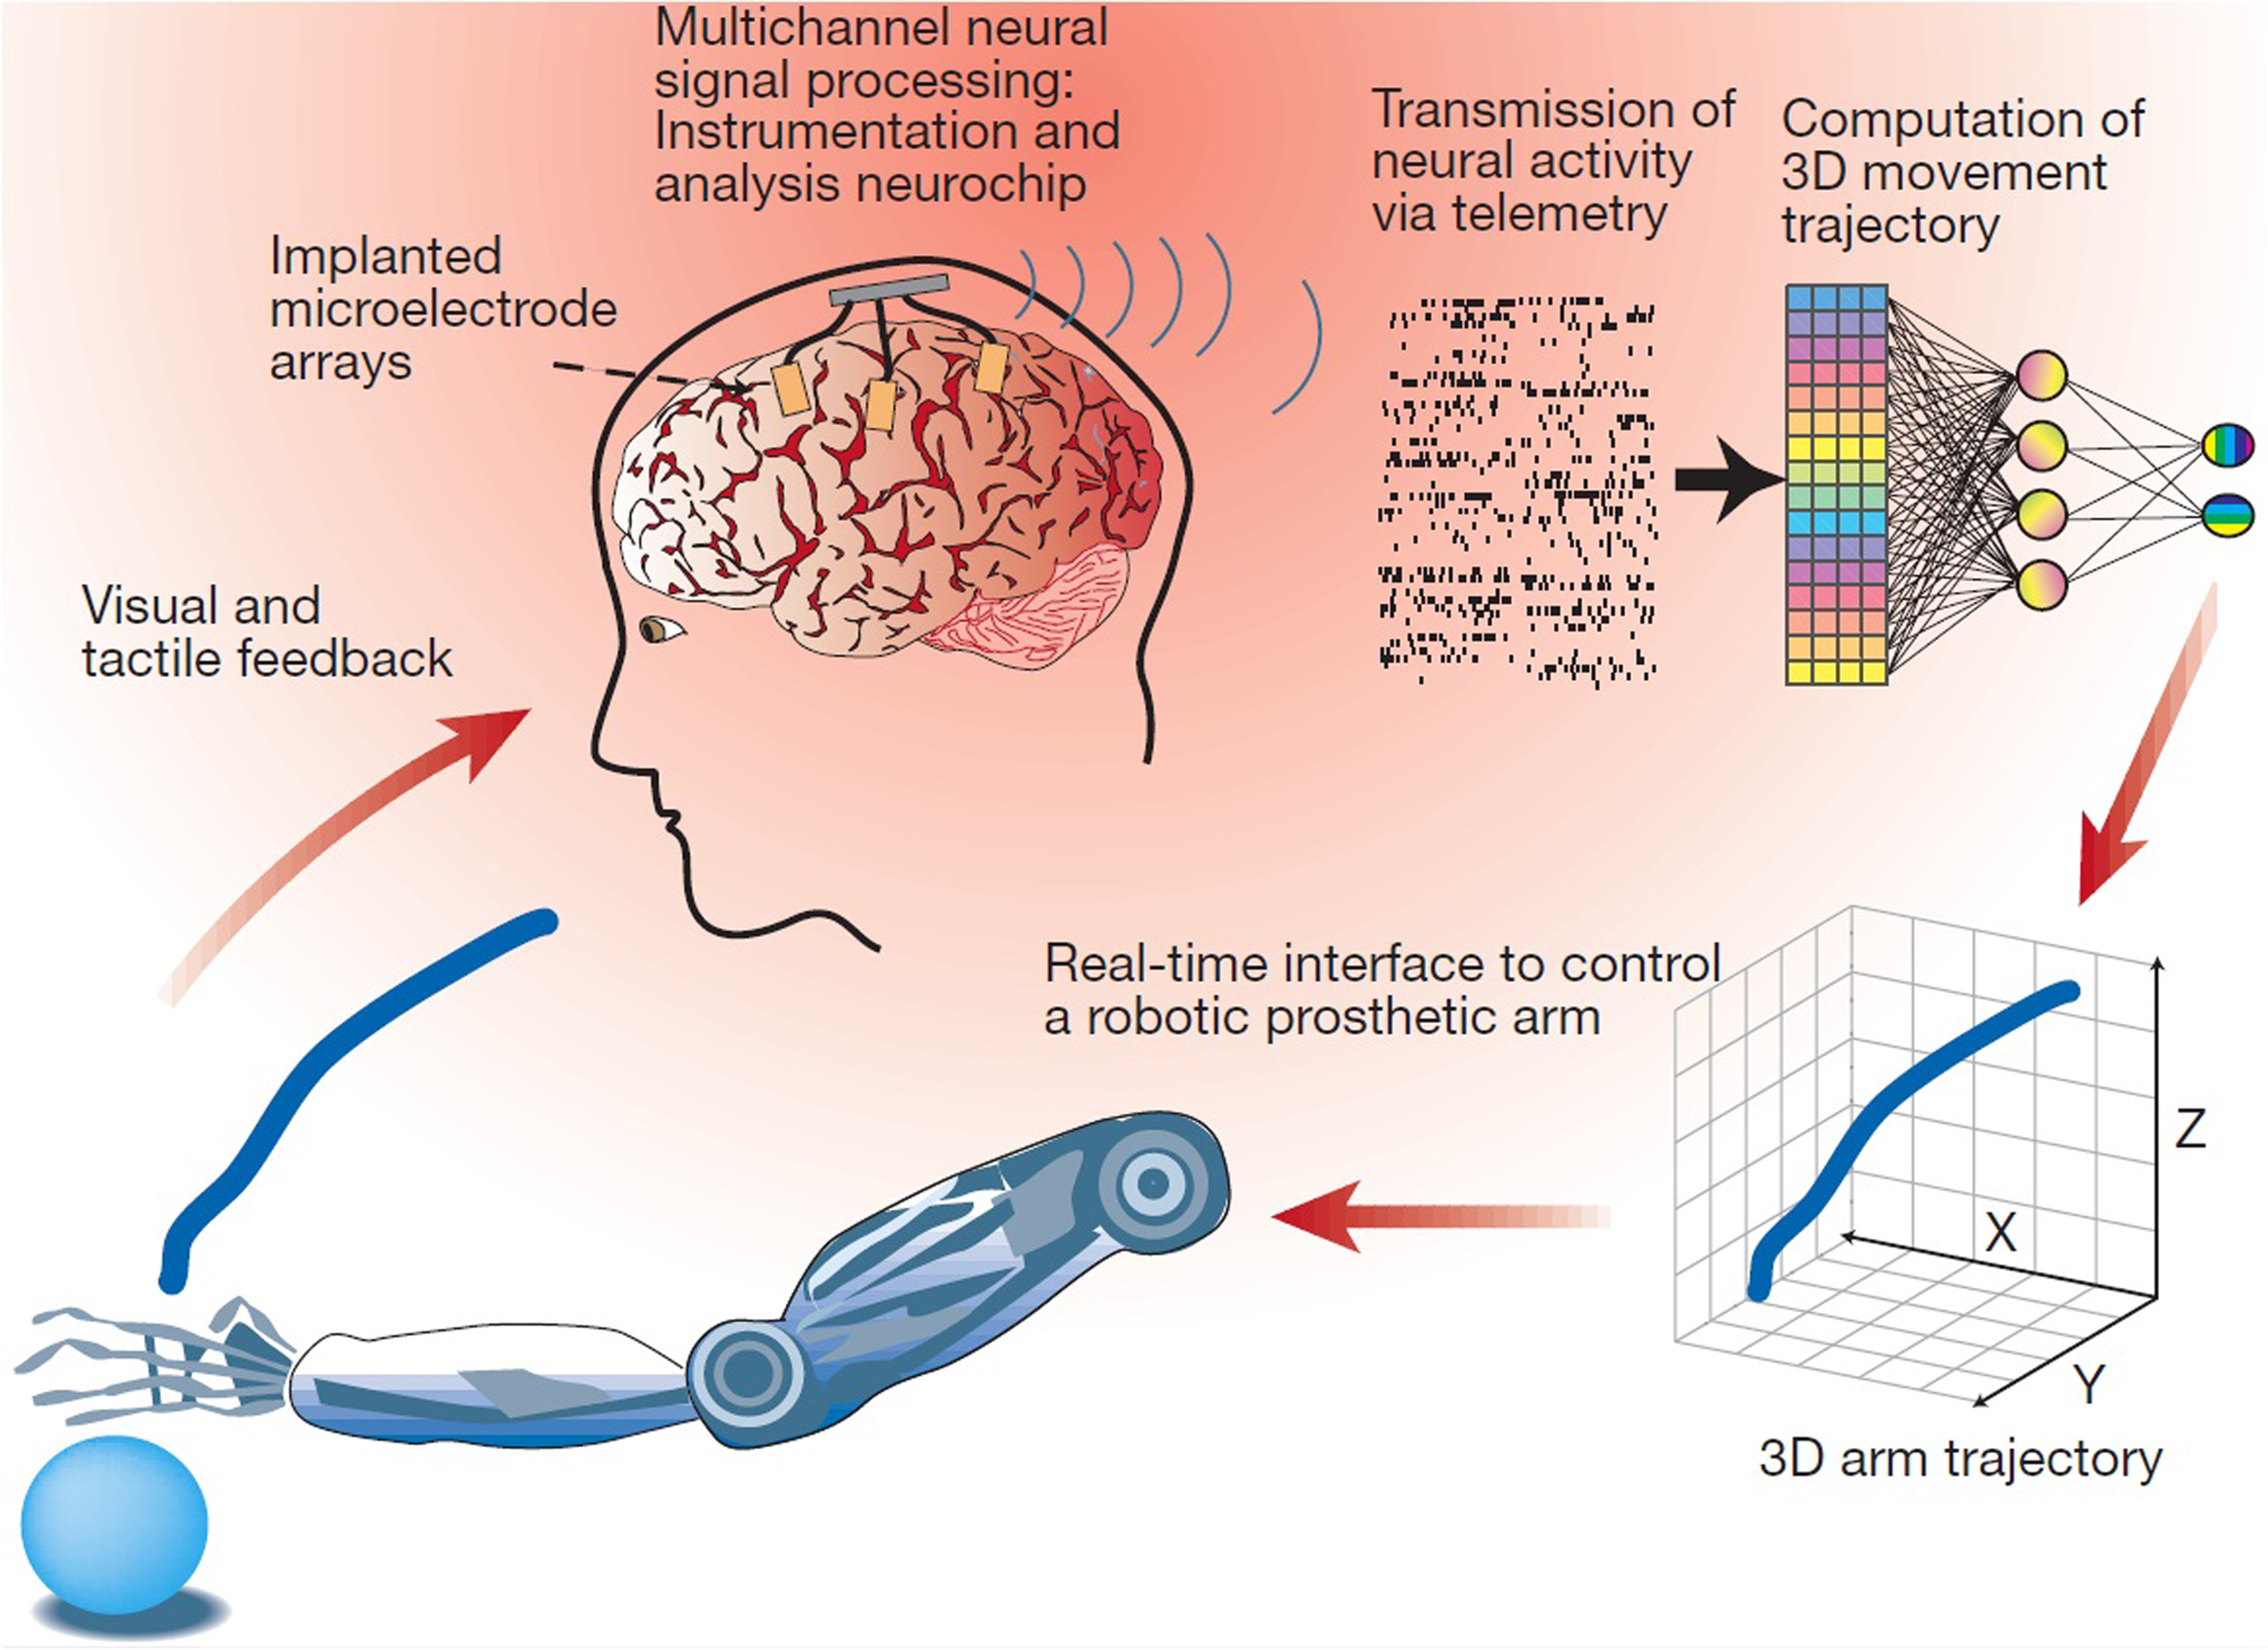
\includegraphics[width=7cm, height=5cm]{fneng-03-00112-g001.jpg}}
\caption{Primena BCI koji koristi ECoG}
\label{Slika}
\end{figure}\\
BCI baziran na ECoG-u može dopustiti korisniku da kontroliše protetičku ruku ili da odabere karaktere koristeći motorne slike ili P300 potencijal u vezi sa doga\dj ajima. Pokazano je da epiduralni ECoG može obezbediti BCI kontrolu, da performans BCI-a baziranog na ECoG-u sa fiksiranim parametrima bude stabilan najmanje 5 dana i da motorne slike – bazične BCI kontrole koje koriste lokacije na motornom korteksu, naprave veće ECoG promene nego one koje su napravljene pravim pokretima. Svi ovi rezultati ukazuju da će se ECoG najverovatnije pokazati praktičnim za dugotrajnu BCI upotrebu.
\\
\section{BCI u svetu gejminga}
Kontekst video igre dodaje mnogo novih izazova za BCI istraživačku zajednicu, i fizička i virtuelna okruženja su veoma složena. Tipičan gejmer je zdrav korisnik, koji može proizvesti širok spektar pokreta tokom igranja, ali većina njih ometaju rad BCI-a. Virtuelno okruženje tako\dj e može ometati upotrebu BCI-a, jer proizvodi mnoge smetnje kao što su vizuelne, taktilne I slušne draži.  Uprkos ovim izazovima video igre imaju veliki potencijal za upotrebu BCI tehnologije, jer imaju za cilj da zabave I motivišu korisnika. Kako motivacija igra glavnu ulogu u uspehu BCI interakcije, video igre predstavljaju veoma relevantno polje primene za obuku i savladavanje BCI sistema. Brojne studije su pokazale kako korišćenje virtuelne realnosti u povratnim informacijama BCI-a poboljšava performanse sistema posebno kod neobučenih korisnika. Upotrebom jeftinih EEG uređaja, korišćenje BCI tehnologije za gejming moguće je i van laboratorije.\\
\begin{figure}[htp]
\centerline{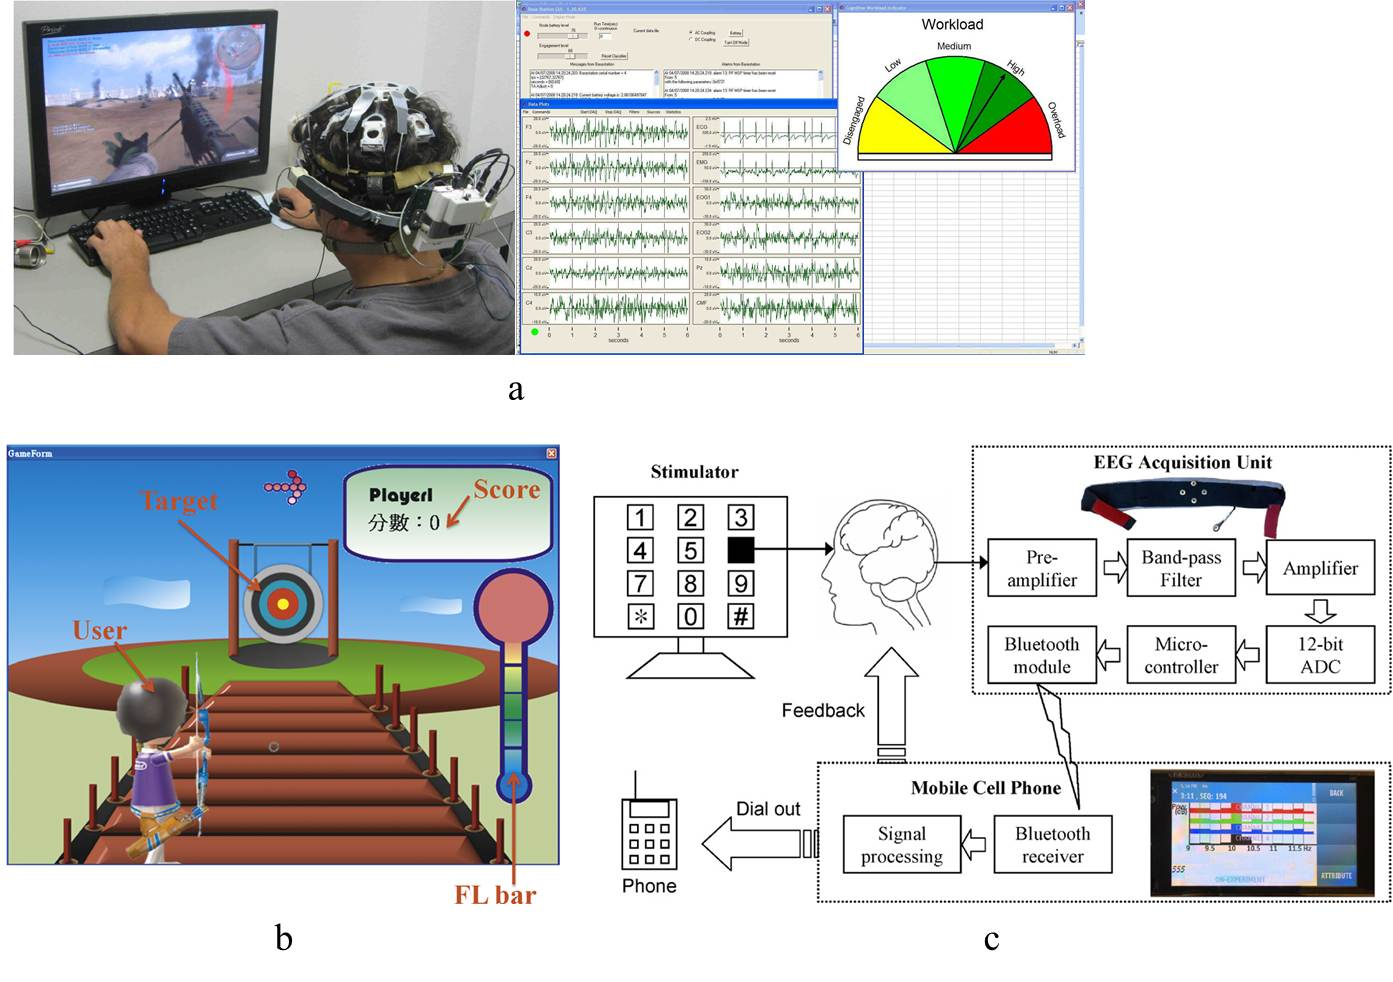
\includegraphics[width=7cm, height=5cm]{image4.jpg}}
\caption{BCI sistem u gejmingu}
\label{Slika}
\end{figure}

Dok je korišćenje BCI za merenje mentalne aktivnosti najkorisniji način da se BCI-i primene u video igrama, danas se koristi i novi načini tj. korišćenje BCI-a kao tradicionalni gejming džojstik. Da bi radio kao džojstik predvi\dj anja BCI-a moraju biti prevedena u smislene komande na način koji omogućava tečno igranje. Ovo implicira da komande moraju da rade u tačnoj vremenskoj skali, da se izdaju sa minimalnim kašnjenjima i da su nepromenljive u odnosu na promene u korisničkom stanju. Vremenska skala u kojoj se izdaju komande treba da bude u skladu sa igrom. Na primer, u igrama sporijeg tempa manje komandi se izdaje tokom jedinice vremena a BCI izlaz se može interpretirati na sličan spor način filtriranjem brzih promena. Igra bržeg tempa može zahtevati brze odgovore pa su stoga za kontrolu potrebni kratki skokovi na izlazu. Neke BCI karakteristike su pogodnije za sporije igre (senzomotorno-korteksni ritmovi), druge su pogodnije za brze akcije (potencijal lateralizovane spremnosti). Primer igre koja zahteva rad u malom vremenskom okviru je Pakman. Kontrola u ovoj igrici analizira se korišćenjem potencijala lateralizovane spremnosti. Za ovu igru, više komandi se obično izdaje u roku od jedne sekunde. Ovo zahteva BCI koji može brzo da reaguje, ali je neosetljiv na promene koje se dešavaju na minutnoj skali.\\
\begin{figure}[htp]
\centerline{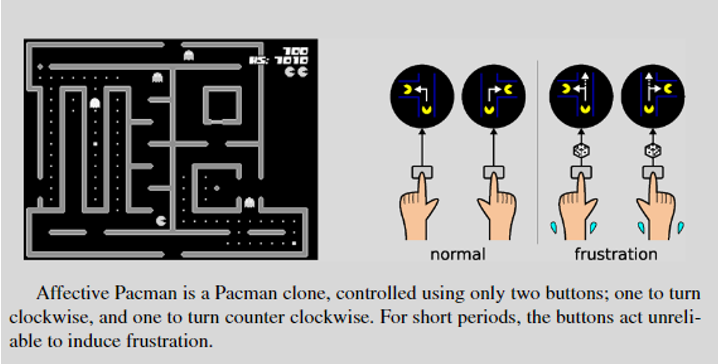
\includegraphics[width=7cm, height=4cm]{pacman.png}}
\caption{Pakman-kontrola igre}
\label{Slika}
\end{figure}\\
Određena latencija je svojstvena kontroli BCI, jer moždane signale treba posmatrati tokom perioda pre nego što se mogu analizirati. Ali za neke karakteristike kao što je potencijal lateralizovane spremnosti za stvarno kretanje, priprema se može posmatrati pre nego što se stvarna radnja dogodi.  Za sporije karakteristike jedino rešenje može biti da se komanda uklopi u istoriju igre što rezultira samo vizuelnim kašnjenjem. Prevođenje radnog BCI-a na smislene komande biće najizazovniji I najvažniji aspekt izgradnje BCI za gejming. \\
\begin{figure}[htp]
\centerline{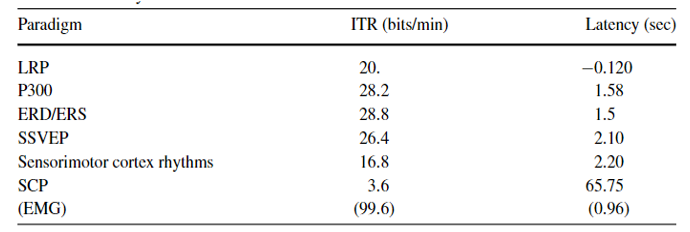
\includegraphics[width=8cm, height=3cm]{brzine.png}}
\caption{Brzine prenosa informacija karakteristika BCI-a}
\label{Slika}
\end{figure}\\
Korišćene BCI zasnovih na EEG-u u kombinaciji sa drugim signalima predstavlja nekoliko dodatnih izazova zbog prirode EEG-a. Jedan od ovih problema su EEG senzori koji imaju tendenciju da pokupe I druge električne signale. Primer takvog signala je električna aktivnost izazvana pokretima očiju ili električna aktivnost usled kontrakcije mišića. Naročito BCI zasnovani na potencijalima mogu patiti od velike promene amplitude uzrokovane pokretima očiju i treptajem oka. Još jedan od izazov sa kojim će se BCI suočiti kada se primeni na igre je uticaj govora i pokreti lica. EMG signal, koji karakteriše signal velike snage u širokom frekvencijskom opsegu ima dubok uticaj na EEG snimke. Dok je govor i izraze lice lakše potisnuti nego pokrete očiju, poželjniji je BCI koji može da radi kompaktno, dok se igrač smeje I priča. \\
Upotrebljivost i korisničko iskustvo koji leže u interakciji između čoveka I računara treba uzeti u obzir prilikom projektovanja sistema i aplikacija, kako bi se povećalo zadovoljstvo korisnika i prihvatanje ove nove tehnologije. 
\section{Zaključak}
Mnogi istraživači  širom sveta razvijaju BCI sisteme koji su pre nekoliko godina bili u domenu naučne fantastike. Ovi sistemi koriste različite moždane signale, metode snimanja i algoritme za obradu signala. Oni mogu da upravljaju mnogim različitim ure\dj ajima, od kursora na ekranima kompjutera do invalidskih kolica i robotskih ruku. Nekoliko osoba sa teškim invaliditetom već koriste BCI za osnovnu komunikaciju i kontrolu u svom svakodnevnom životu. Sa boljim hardverom za akviziciju signala, jasnom kliničkom validacijom, i ono što je najvažnije a to je povećanje pouzdanosti, BCI mogu postati nova glavna tehnologija komunikacije i kontrole za osobe sa invaliditetom, a možda i za opštu populaciju tako\dj e.

\nocite{*}
\bibliographystyle{plain}
\bibliography{mybibliography.bib}



\end{document}

